\section{Résultats}

\subsection{Benchmarks}
Nous avons implémenté les algorithmes en langage Rust et le code source est disponible sur Gitlab.
Pour chaque taille de mot $n = |a| = |b|$ indiquée, 
nous avons effectué l'expérience suivante 100 fois : nous avons choisi des mots aléatoires $a, b \in A$ de longueur $n$, 
avons défini $c = ab$, puis avons appliqué l'Algorithme 1 à $c$ et $b$. Pour chaque valeur de $N$ et de $n$, 
nous avons trouvé le temps d'exécution médian nécessaire pour trouver une solution. 
Dans tous les cas, les solutions ont été vérifiées pour être correctes. \\
\begin{figure}[!ht]
	\centering
	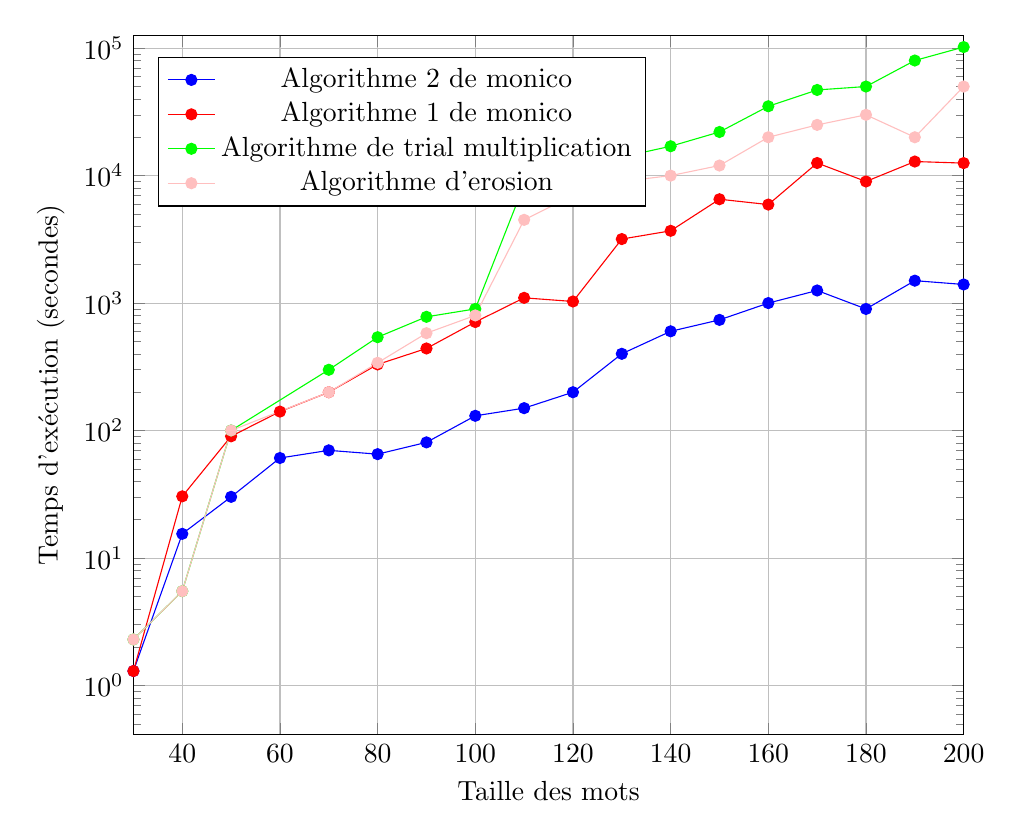
\begin{tikzpicture}
	\begin{axis}[
		xlabel={Taille des mots},
		ylabel={Temps d'exécution (secondes)},
		legend pos=north west,
		grid=major,
		ymin=0,
		xmin=30,
		ymax=125400,
		xmax=200,
		width=\textwidth,
		ymode=log,
	]
	
	\addplot[color=blue,mark=*] coordinates {
		(30, 1.3)
		(40, 15.5)
		(50, 30.22)
		(60, 60.96)
		(70,70)
		(80,65.35)
		(90,80.85)
		(100,130.64)
		(110, 150)
		(120, 200)
		(130, 400.29)
		(140, 600.94)
		(150, 738.70)
		(160, 1000.69)
		(170, 1256.17)
		(180, 900)
		(190, 1500.05)
		(200, 1400.42)
	};
	\addlegendentry{Algorithme 2 de monico}
	
	\addplot[color=red,mark=*] coordinates {
		(30, 1.3)
		(40, 30.5)
		(50, 90.22)
		(60, 140.96)
		(70,200)
		(80,330.35)
		(90,440.85)
		(100,710.64)
		(110, 1100)
		(120, 1030)
		(130, 3180.29)
		(140, 3690.94)
		(150, 6530.70)
		(160, 5930.69)
		(170, 12560.17)
		(180, 9000)
		(190, 12900.05)
		(200, 12540.42)
	};
	\addlegendentry{Algorithme 1 de monico}
	\addplot[color=green,mark=*] coordinates {
		(30, 2.3)
		(40, 5.5)
		(50, 100.22)
		(70,300)
		(80,540.35)
		(90,780.85)
		(100,900.64)
		(110, 8500)
		(120, 12000)
		(130, 14000.29)
		(140, 17000.94)
		(150, 22000.70)
		(160, 35000.69)
		(170, 47000.17)
		(180, 50000)
		(190, 80000.05)
		(200, 102000.42)
	};
	\addlegendentry{Algorithme de trial multiplication}
	\addplot[color=pink,mark=*] coordinates {
		(30, 2.3)
		(40, 5.5)
		(50, 100.22)
		(70,200)
		(80,340.35)
		(90,580.85)
		(100,800.64)
		(110, 4500)
		(120, 7000)
		(130, 9000.29)
		(140, 10000.94)
		(150, 12000.70)
		(160, 20000.69)
		(170, 25000.17)
		(180, 30000)
		(190, 20000.05)
		(200, 50000.42)
	};
	\addlegendentry{Algorithme d'erosion}
	\end{axis}
	\end{tikzpicture}
	\caption{Benchmark des quatre algorithmes}
	\label{fig:benchmark}
\end{figure}
La figure \ref{fig:benchmark} présente les résultats de notre benchmark sur quatre algorithmes différents.
Le temps d'exécution (en secondes) est représenté en fonction de la taille des mots testés.
\begin{flushleft}
	Les résultats montrent que l'Algorithme 2 de Monico est le plus rapide pour toutes les tailles de mots testées. Les temps d'exécution de cet algorithme augmentent régulièrement avec la taille des mots, mais restent relativement faibles jusqu'à environ $n=80$, puis augmentent plus rapidement par la suite.
	
	L'Algorithme 1 de Monico est plus lent que l'Algorithme 2 pour toutes les tailles de mots testées, mais reste tout de même efficace pour les mots de taille inférieure à environ 80. Au-delà de cette taille, les temps d'exécution augmentent rapidement.
	
	L'algorithme d'érosion est le troisième plus rapide pour les tailles de mots inférieures à environ 70, mais devient rapidement plus lent pour les tailles de mots supérieures.
	
	L'algorithme de trial multiplication est le plus lent de tous les algorithmes testés, mais reste relativement efficace pour les tailles de mots inférieures à environ 80, avant de devenir très lent pour les tailles de mots supérieures.
	
	En somme, le graphique permet de visualiser les performances des quatre algorithmes testés en fonction de la taille des mots.
\end{flushleft}

Notez que le symbole $n$ est utilisé pour représenter la taille des mots, et qu'il doit être écrit en mode mathématique pour apparaître en italique.

\subsection{Challenge de Brown}
Dans son article, Brown propose un challenge qui consiste à résoudre une division issue de la multiplication de deux mots de taille 512 sur un alphabet de 64 symboles. Ceci est impossible avec la division par érosion : il faudrait un temps infini. Les mots que Brown propose de diviser sont construits sur l'alphabet des caractères du standard base64. Nous avons créé des fonctions permettant de passer des mots codées de la sorte aux mots sur l'alphabet des entiers de 1 à 64 dans les deux sens pour pouvoir les utiliser avec notre programme. Avec le code C fournit par Monico, nous avons pu résoudre le challenge en 117,75s. Le meilleur temps que nous ayons obtenu pour résoudre ce challenge avec notre programme sur la même machine est de 579,91s. Cependant, étant donné la grande variabilité sur le temps de résolution dû au non-déterminisme de l'algorithme, il serait plus pertinent de faire de plus nombreux tests et de comparer les temps moyens.

\section{Discussion}
Notre code semble plus lent que celui codé en C par Brown et Monico. Une piste d'amélioration serait donc d'optimiser le code. Pour cela, on peut envisager de changer la façon dont les algorithmes sont implémentés, changer les structures de donnée ou essayer de paralléliser le code. 

Faire davantage de tests, sur des tableaux de tailles plus grandes et en essayant de trouver des caractéristiques des tableaux pouvant influencer le temps d'exécution des divisions serait intéressant. Nous ne l'avons pas fait par manque de temps.

Nous ne savons pas pourquoi le second algorithme de Monico fonctionne mieux que le premier, il serait utile d'avoir une explication à cela pour éventuellement améliorer encore l'algorithme.

Dans l'idéal, il faudrait trouver un algorithme de division polynomial déterministe, pour pouvoir en calculer la complexité théorique et ainsi être définitivement fixé sur la possibilité de l'utilisation du monoïde plaxique pour une application cryptographique.

Dans l'idéal, il faudrait trouver un algorithme de division polynomial déterministe, pour pouvoir en calculer la complexité théorique et ainsi être définitivement fixé sur la possibilité de l'utilisation du monoïde plaxique pour une application cryptographique.